\chapter{Verwandte Arbeiten}
\label{chap:related}

Da in dieser Arbeit verschiedene Forschungsbereiche miteinander kombiniert werden, ist dieses Kapitel in zwei Abschnitte eingeteilt: Es wird mit einigen verwandten Arbeiten im Bereich der Bildsegmentierung begonnen, dabei wird insbesondere auf die Nutzung von neuronalen Netzen eingegangen. Anschließend werden Clusteringprozesse betrachtet, welche zur Initialisierung der Segmentierungsalgorithmen genutzt werden. 

\iffalse
Zuletzt folgt die Analyse der Marsoberfläche, hauptsächlich der Kratererkennung. % TODO Remove mars?
\fi

\section{Bildsegmentierung}
\label{sec:image_segmentation}

\subsection{DEC -- Deep Embedded Clustering}
\label{ssec:dec}
In \cite{junyuan_16} wird eine Methode zur Bildsegmentierung durch neuronale Netze ohne vorherige Ground Truth vorgestellt: Das Ziel besteht daraus, $N$ Punkte $\{x_n\in X\}_{n=1}^N$ in $k$ verschiedene Cluster mit den jeweiligen Clusterzentren $\mu_j, j\in\left[1, k\right]$ einzuteilen. Entgegen des naiven Ansatzes, direkt die Farbwerte der einzelnen Pixel als Merkmalsraum $X$ zu nutzen und zu clustern, wird in \cite{junyuan_16} nicht direkt anhand der Farbwerte geclustert, stattdessen wird dieser zuerst über eine nichtlineare Funktion $f_\theta: X\rightarrow Z$ in einen Merkmalsraum $Z$ abgebildet. $\theta$ ist dabei ein erlernbarer Parameter, sodass das genutzte Neuronale Netz zwei Parameter zeitgleich optimiert: $\theta$, und die Position der Clustermitten $\mu_j$.

Der DEC-Algorithmus besteht aus zwei Phasen:
\begin{enumerate}
	\item{Parameterinitialisierung:}\\
	Um die Startparameter für $\theta$ zu Generieren wird ein Stacked Autoencoder (SAE, \cite{vincent_10}) schichtenweise aufgebaut. Jede Schicht des SAEs ist ein rauschunterdrückender Autoencoder, welcher wie folgt definiert ist: \cite{junyuan_16}
	\begin{eqnarray}
	\bar{x}&\sim&Dropout(x)\\
	h &=& g_1(W_1\tilde{x}+b_1)\\
	\tilde{h} &\sim& Dropout(h)\\
	y &=& g_2(W_2\tilde{h}+b_2)
	\end{eqnarray}
	Zuerst wird ein Encoder-Decoder-Paar dazu trainiert, ein Signal wiederherzustellen, nachdem dieses eine Encoder-Schicht durchlaufen hat. Anschließend wird der Parameter $h$ dazu genutzt, ein weiteres Paar zu trainieren (\vgl \figurename~\ref{fig:sae}). Am Ende dieses Lernens besteht $\theta$ aus der Menge aller Gewichtungen $W$ und Bias $b$ der verschiedenen Encoder Schichten. Diese Encoder-Schichten beschreiben nun die Funktion $f_\theta$, welche den originalen Merkmalsraum $X$ des Bildes in den reduzierten Merkmalsraum $Z$ umwandelt.
	
	Die initialen Clustermitten werden durch den k-Means-Algorithmus auf dem Merkmalsraum $Z$ generiert.
	
	\item{Parameteroptimierung:}\\
	Das eigentliche Lernen des DEC-Algorithmus findet in zwei, sich gegenseitig abwechselnden Phasen statt:
	
	Zuerst wird eine Zuweisung von den Datenpunkten des Merkmalsraumes zu den Koordinaten der Clusterzentren berechnet. Zu diesem Zweck wird eine Wahrscheinlichkeitsverteilung, die t-Verteilung genutzt:
	
	\begin{equation}
		f(t)=\frac{\Gamma\left(\frac{\nu+1}{2}\right)}{\sqrt{\nu\pi}\Gamma\left(\frac{\nu}{2}\right)}\left(1+\frac{t^2}{\nu}\right)^{-\frac{\nu+1}{2}}
	\end{equation}
	
	Dabei ist $\Gamma$ die Gamma-Funktion und $\nu$ die Anzahl der Freiheitsgrade.
	
	Diese Funktion berechnet also die Wahrscheinlichkeit, dass ein bestimmter Datenpunkt einem bestimmten Cluster zugewiesen wird.
	
	Anschließend werden die Positionen der Clustermitten $\mu_j$ und die Parameter $\theta$ der Funktion $f_\theta$ optimiert. Die zu verringernde Verlustfunktion ist an dieser Stelle die Kullback-Leibler-Divergenz. Somit wird hier eine Funktion gelernt, welche sich möglichst wenig von der oben beschriebenen, iterativ generierten $t$-Verteilung unterscheidet. Der eigentliche Optimierungsprozess der Clustermitten und der Parameter für $\theta$ findet über das Gradientenverfahren (\vgl Unterabschnitt~\ref{ssec:gradient_descent}) statt.
\end{enumerate}

\begin{figure}[h!]
	\centering
	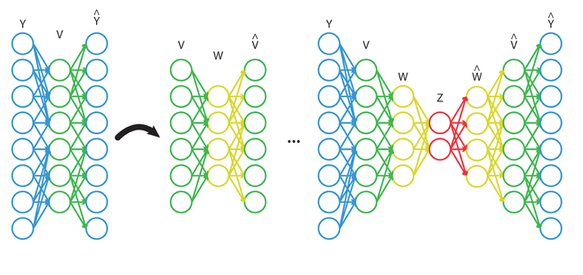
\includegraphics[width=.8\textwidth,keepaspectratio]{images/BK15/BK15_01.png}
	\caption{Initialisierung eines Stacked Autoencoders, modifiziert, aus \cite{berniker_15}. Zu Beginn existiert ein Encoder-Paar (blau) bestehend aus Encoder $Y$ und Decoder $\hat{Y}$ mit einer Zwischenausgabe $V$ (links). Anschließend wird diese Ausgabe $V$ dazu genutzt, ein weiteres Autoencoder-Paar so zu trainieren, dass es die Eingabe $V$ durch $\hat{V}$ approximieren kann (mitte). Dies geschieht iterativ so lange, bis die Anzahl der gewünschten Schichten erreicht ist. Zuletzt werden die so generierten Autoencoder-Paare verschachtelt (rechts).}
	\label{fig:sae}
\end{figure}

Zusammengefasst lernt der Algorithmus in der ersten Phase seiner Ausführung, wie er nach der Anwendung von Dropout-Schichten die ursprüngliche Eingabe bestmöglich wiederherstellen kann, er lernt also wie signifikant bestimmte Merkmale zur Wiederherstellung sind. Diese Initialisierung wird im zweiten Schritt weiter optimiert.
Der Vorteil dieser und ähnlicher Methoden besteht daraus, dass das Netzwerk nicht trainiert werden muss und somit also auch keine Ground Truth benötigt. Dies ermöglicht dessen Einsatz in Bereichen in denen es zu aufwändig ist, Ground Truths manuell zu erstellen. Eine weitere Eigenschaft besteht daraus, dass diese Methode sich für den Einsatz auf unterschiedlichsten Eingabedaten eignet, da sie dynamisch zur Laufzeit lernt, nach welchen Kriterien sie clustern sollte.
% TODO Initialisierung Abbruchkriterium

\subsection{Bildsegmentierung auf Basis eines Bildclusterings}
\label{ssec:kanezaki}
Ein vergleichbarer, wenn auch einfacherer Ansatz wird in \cite{kanezaki_18} beschrieben. Auch dieser Ansatz erstellt eine Mapping-Funktion $c_n=f(x_n)$, die jedem der $N$ $p$-dimensionalen Pixel mit dem Merkmalsvektor $\{x_n\in\mathbb{R}^p\}_{n=1}^N$ eines Eingabebildes ein Clusterlabel $c$ mit $\{c_n\in\mathbb{Z}\}_{n=1}^N$ zuordnet. Anders als beim DEC-Algorithmus wird aber auf Autoencoder verzichtet und zusätzlich direkt im Merkmalsraum der Farbwerte geclustert.

Statt das neuronale Netz selbst eine Initialisierung lernen zu lassen, wird in diesem Algorithmus auf Clusteringalgorithmen aus der Bildverarbeitung zurückgegriffen, insbesondere wird der SLIC-Algorithmus \cite{achanta_10} genutzt.

Eine Segmentierung wird durch einen iterativen Prozess erreicht, in welchem ein anfangs untrainiertes neuronales Netz eine Bildsegmentierung erzeugt, welche anschließend mithilfe der im Vorhinein erstellten, konstanten Segmentierung optimiert wird. Diese Optimierung besteht daraus, dass für jedes Cluster des SLIC-Algorithmus überprüft wird, welches Label das neuronalen Netz am häufigsten den Pixeln im Cluster zugewiesen wurde. Anschließend wird jedes Cluster mit eben diesem häufigsten Label gefüllt und die Differenz zwischen der Ausgabe des Netzwerkes und diesem neu generierten \enquote{Ziel} betrachtet.
Der gesamte Algorithmus ist in \figurename~\ref{fig:Kan18_01} dargestellt, eine genauere Beschreibung findet sich in Abschnitt~\ref{sec:howitworks}.

\begin{figure}[h!]
	\centering
	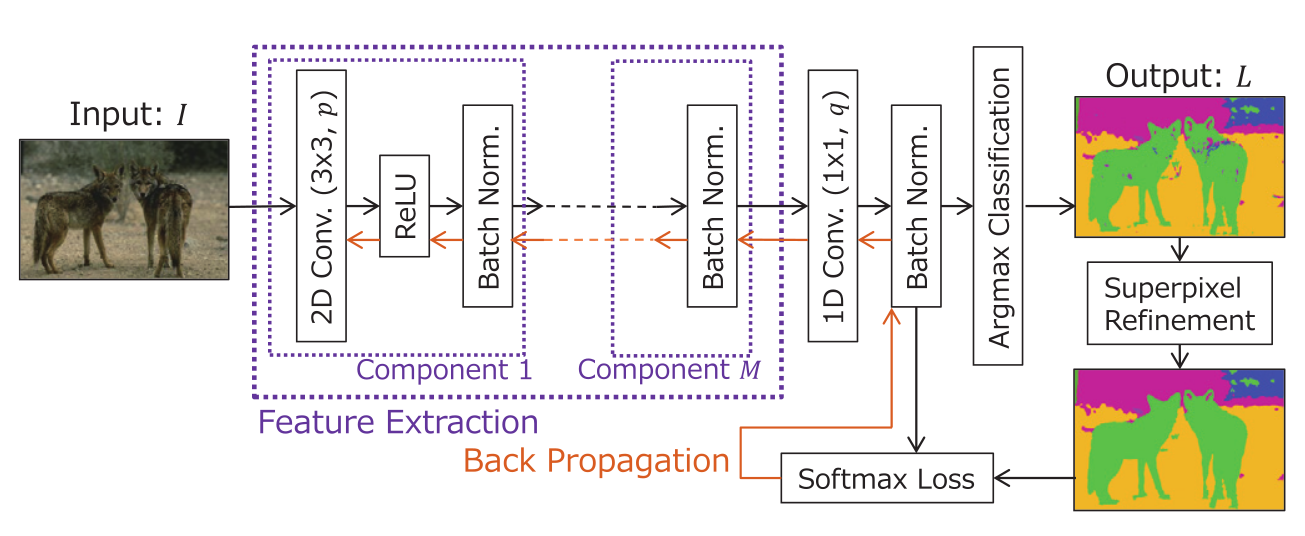
\includegraphics[width=.8\textwidth,keepaspectratio]{images/Kan18/Kan18_01.png}
	\caption{Vorgehensweise nach Kanezaki, aus \cite{kanezaki_18}}
	\label{fig:Kan18_01}
\end{figure}

Es gilt zu beachten, dass zur Initialisierung ein möglichst feines Clustering genutzt wird, da im Laufe des Prozesses mehrere einzelne Cluster miteinander vereint werden, bis die gewünschte Anzahl an Segmenten erreicht wird.

Insgesamt lernt dieser Algorithmus iterativ die Ausgabe der Clusteringfunktion anzunähern, mit dem Unterschied, dass er in diesem Prozess mehrere Clusterzentren miteinander vereinen kann. Da in \cite{kanezaki_18} auf Basis des SLIC-Algorithmus gearbeitet wird, lernt das neuronale Netz hauptsächlich anhand der Farbwerte einzelner Pixel und deren Entfernungen zu ähnlichen Pixeln, wie es eine Eingabe segmentieren soll. Damit kann es als eine vereinfachte Version des DEC-Algorithmus betrachtet werden, da dieser dynamisch bestimmt, Anhand welcher Merkmale das Clustering geschehen soll.

\section{Bildclustering}
\label{ssec:clustering}

Der in Unterabschnitt~\ref{ssec:kanezaki} vorgestellte Algorithmus benötigt zur Initialisierung ein relativ feines Clustering der Eingabedatei. Erreicht wird dieses Über den SLIC Superpixel Algorithmus. Dieser besteht aus der Anwendung des k-Means Algorithmus auf einem fünfdimensionalen Merkmalsraum, bestehend aus drei Dimensionen für die jeweiligen Farbwerte eines Pixels im CIELAB Farbraum und zwei Dimensionen für die X- und Y-Koordinaten des Pixels. \cite{achanta_10} Der k-Means-Algorithmus teilt eine beliebige Anzahl von Messpunkten (in diesem Fall je ein Merkmalsvektor pro Pixel) in eine vorher festgelegte Menge an Clustern ein.

Dieser Algorithmus ist weitverbreitet und liefert oft gute Ergebnisse auf unterschiedlichen Eingaben, er eignet sich allerdings nur bedingt um Graustufenbilder zu clustern. Da nicht garantiert ist, dass Eingabedateien mehrfarbig sind, eignet sich eine farbbasierte Clustering-Methode wie SLIC nicht immer um diese zuverlässig zu clustern. 

Des Weiteren liefert SLIC bei Eingaben in denen ein Segment starke Hell-/Dunkel-Differenzen besitzt keine optimalen Ergebnisse, da es primär anhand der Farbwerte \bzw Helligkeitswerte clustert. Diese Problematik ist genauer in Abschnitt~\ref{sec:initialization} beschrieben.

\subsection{Texturbasiertes Clustering}
\label{ssec:tsugf}

Neben dem farbbasierten Clustering existiert auch das texturbasierte Clustering. Bei diesem werden weniger die Farbwerte von benachbarten Pixeln, sondern vielmehr die Texturen in benachbarten Bereichen verglichen.

Eine Methode des texturbasierten Clusterings wird in \cite{jain_91} beschrieben: Dort wird eine Reihe von Gabor-Filtern dazu benutzt, die Textur des Bildes zu analysieren. Dieser Prozess verläuft wie folgt:

Zuerst wird eine Reihe von Gabor-Filtern --~auch Filterbank genannt~-- erstellt. Ein Beispiel, welches nach der originalen Ausarbeitung nachgestellt wurde, findet sich in \figurename~\ref{fig:tsugf_filters}. Es gilt zu beachten dass jeder Filter in mehrmals in unterschiedlichen Größen erstellt wird.

\begin{figure}[h!]
	\centering
	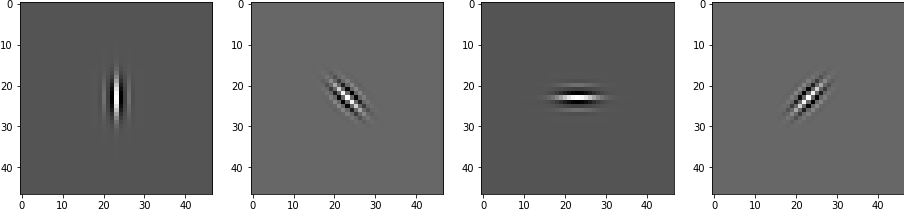
\includegraphics[width=0.5\textwidth,keepaspectratio]{images/gen/tsugf_filters/filters.png}
	\captionsetup{width=0.5\textwidth,format=plain}
	\caption{Zum texturbasierten Clustering genutze Filterbank}
	\label{fig:tsugf_filters}
\end{figure}

Diese werden anschließend über das in den Unterabschnitten~\ref{ssec:convolution} und \ref{ssec:convolutional_layer} beschriebene Konvolutionsverfahren angewandt. Dieser Vorgang resultiert in einem Datenwürfel, bei welchem die ersten beiden Dimensionen gleich der Höhe und Breite der Eingabebilddatei sind, und die dritte Dimension gleich der Anzahl der genutzten Filter ist. Somit enthält jede Schicht des Würfels Informationen darüber, wie sehr und wo im Bild das Muster der jeweiligen Filterbank \enquote{erkannt} wird. Dies ist in \figurename~\ref{fig:tsugf_101027_raw} sichtbar.

\begin{figure}[h!]
	\begin{subfigure}[t]{0.32\textwidth}
		\centering
		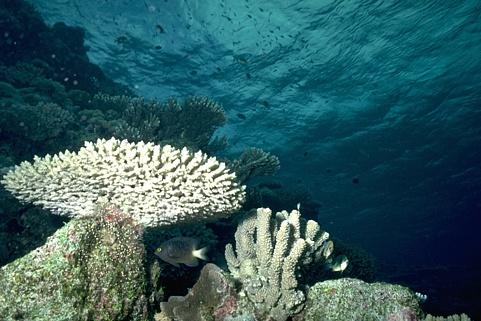
\includegraphics[width=\textwidth,keepaspectratio]{images/bsd/101027.jpg}
		\captionsetup{format=plain}
		\subcaption{}
		\label{fig:bsd_101027}
	\end{subfigure}
	\hfill
	\begin{subfigure}[t]{0.32\textwidth}
		\centering
		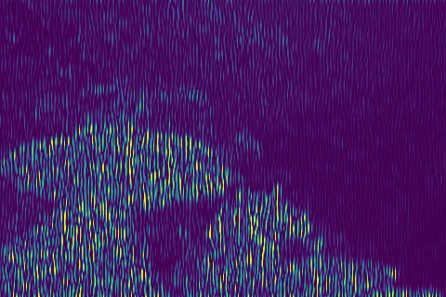
\includegraphics[width=\textwidth,keepaspectratio]{images/gen/convolution/101027.jpg_0.png}
		\subcaption{}
	\end{subfigure}
	\hfill
	\begin{subfigure}[t]{0.32\textwidth}
		\centering
		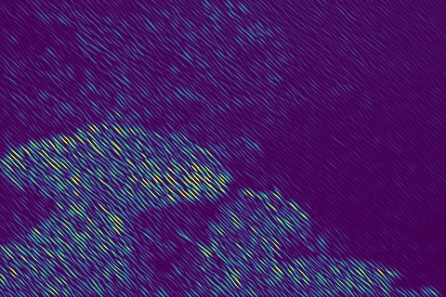
\includegraphics[width=\textwidth,keepaspectratio]{images/gen/convolution/101027.jpg_1.png}
		\subcaption{}
	\end{subfigure}
	\hfill
	\begin{subfigure}[t]{0.32\textwidth}
		\centering
		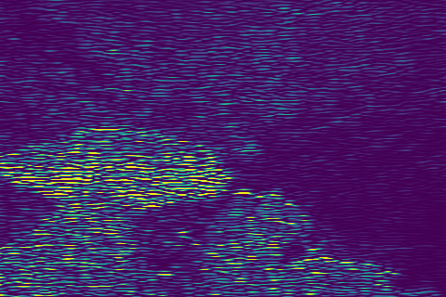
\includegraphics[width=\textwidth,keepaspectratio]{images/gen/convolution/101027.jpg_2.png}
		\subcaption{}
	\end{subfigure}
	\hfill
	\begin{subfigure}[t]{0.32\textwidth}
		\centering
		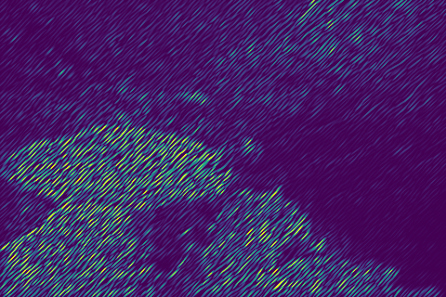
\includegraphics[width=\textwidth,keepaspectratio]{images/gen/convolution/101027.jpg_3.png}
		\subcaption{}
	\end{subfigure}
	\hfill
	\begin{subfigure}[t]{0.32\textwidth}
		\hfill
	\end{subfigure}
	\caption{Ergebnisse (b-e) der Konvolution des Beispielbildes (a, aus \cite{bsd500}) mit den jeweiligen Filtern}
	\label{fig:tsugf_101027_raw}
\end{figure}

Ähnlich zur Vorgehensweise von SLIC wird dem werden dem Datenwürfen zusätzliche Informationen über die jeweiligen X- und Y-Koordinaten hinzugefügt. Anschließend wird der k-Means-Algorithmus auf diesen Datenwürfel angewandt, es werden also Pixel mit ähnlichen Texturen und geringer Distanz zueinander in Cluster zusammengefasst.

In der Praxis sind für die erfolgreiche Anwendung dieser Methode allerdings noch einige Optimierungen notwendig: \cite{mathworks_15}

\paragraph{Weichzeichnung}
Da die Anwendung des Konvolutionsverfahrens wie in \figurename~\ref{fig:tsugf_101027_raw} sichtbar zu einer streifenartigen Merkmalsextraktion führen kann, macht es in vielen Fällen Sinn, die jeweiligen Merkmalsebenen weichzuzeichnen. Als Radius eignet sich hier ein Wert, welcher groß genug ist um die Streifen zu entfernen, aber klein genug ist, als dass die Ränder der jeweiligen erkannten Texturen nicht in benachbarte Texturen überfließen.
\paragraph{Räumlicher Bezug}
Damit diese Cluster eine (bessere) räumliche Beziehung zueinander haben, wird zu den Merkmalsdimensionen je eine Schicht hinzugefügt, welche ausschließlich mit den X-Koordinaten der jeweiligen Pixel gefüllt ist. Selbiges geschieht für die jeweiligen Y-Koordinaten. Da diese vom k-Means Algorithmus auch zusammen geclustert werden, entsteht ein örtlicher Bezug unter den Clustern. Dies wurde auch in der ursprünglichen Ausarbeitung \cite{jain_91} berücksichtigt.
\paragraph{Normalisierung}
Die jeweiligen Schichten sollten vor der Anwendung des k-Means-Algorithmus normalisiert werden um zu vermeiden, dass manche Merkmale stärer gewichtet werden als andere. Dies ist insbesondere wichtig, wenn wie oben genannt die Farb- oder Positionswerte den Merkmalsdimensionen hinzugefügt werden, da diese sich oft auf unterschiedlichen Skalen gegenüber den Konvolutionsergebnissen befinden.
\paragraph{Farbdimensionen}
Wenn die Eingabedatei eine RGB-Aufnahme ist, können diese drei Farbkanäle zur besseren Unterscheidung von unterschiedlichen Clustern mit ähnlichen Texturen genutzt werden. Dazu wird die Aufnahme in ihre drei Farbkanäle aufgeteilt und diese drei Schichten anschließend als Merkmalsdimensionen dem Datenwürfel hinzugefügt. Obwohl dies nicht in \cite{jain_91} aufgeführt wird, ist es in manchen Anwendungsbereichen zur gängigen Praxis geworden.

\paragraph{}
Das schrittweise Hinzufügen dieser Optimierungen ist in \figurename~\ref{fig:tsugf_optim} sichtbar.

\begin{figure}[h!]
	\begin{subfigure}[t]{0.32\textwidth}
		\centering
		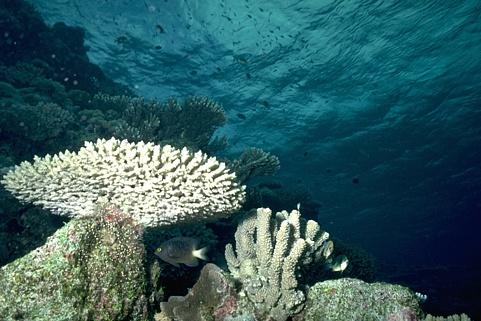
\includegraphics[width=\textwidth,keepaspectratio]{images/bsd/101027.jpg}
		\subcaption{Beispielbild (aus \cite{bsd500})\\\xspace}
	\end{subfigure}
	\hfill
	\begin{subfigure}[t]{0.32\textwidth}
		\centering
		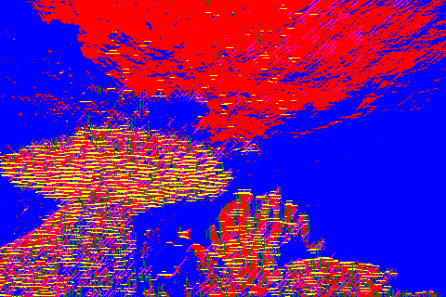
\includegraphics[width=\textwidth,keepaspectratio]{images/gen/optims/101027.jpg_raw.png}
		\captionsetup{format=plain}
		\subcaption{Originales Clusteringergebnis\\\xspace}
	\end{subfigure}
	\hfill
	\begin{subfigure}[t]{0.32\textwidth}
		\centering
		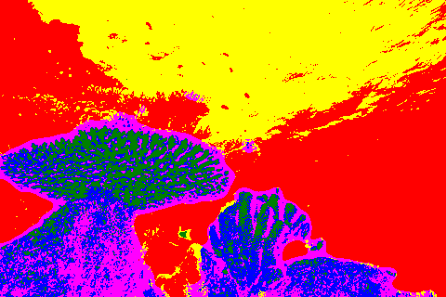
\includegraphics[width=\textwidth,keepaspectratio]{images/gen/optims/101027.jpg_blur.png}
		\subcaption{Weichzeichnen der Konvolutionsergebnisse}
	\end{subfigure}
	\hfill
	\begin{subfigure}[t]{0.32\textwidth}
		\centering
		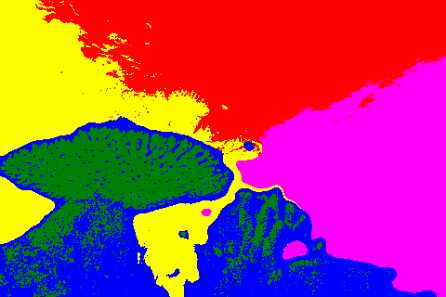
\includegraphics[width=\textwidth,keepaspectratio]{images/gen/optims/101027.jpg_blur_norm_spatial.png}
		\subcaption{Zusätzliche räumliche Informationen und Normierung}
	\end{subfigure}
	\hfill
	\begin{subfigure}[t]{0.32\textwidth}
		\centering
		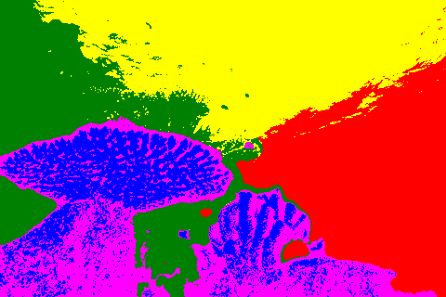
\includegraphics[width=\textwidth,keepaspectratio]{images/gen/optims/101027.jpg_blur_norm_spatial_color.png}
		\subcaption{Zusätzliche Farbinformationen}
	\end{subfigure}
	\hfill
	\begin{subfigure}[t]{0.32\textwidth}
		\hfill
	\end{subfigure}
	\caption{Optimierung des Clusteringverfahrens}
	\label{fig:tsugf_optim}
\end{figure}

Neben der in \figurename~\ref{fig:tsugf_filters} gezeigten Filterbank existieren alternative Filterbänke, \ua:
\begin{itemize}
	\item Die Leung-Malik (LM) Filterbank \cite{leung_01}
	\item Die Schmid (S) Filterbank \cite{schmid_01}
	\item Die Maximum Response (MR) Filterbank \cite{visgeo}
\end{itemize}

Diese drei Filterbänke besitzen im Gegensatz zu der in \cite{mathworks_15} vorgestellten Filterbank auch Filter in verschiedenen Größen und rotationsinvariante Filter. Sie sind in \figurename~\ref{fig:filterbank} dargestellt.

\begin{figure}[h!]
	\begin{subfigure}[t]{0.38\textwidth}
		\centering
		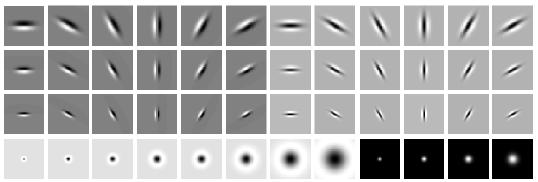
\includegraphics[width=\textwidth,keepaspectratio]{images/vis/vis_01.jpg}
		\captionsetup{format=plain}
		\subcaption{Leung-Malik-Filterbank}
	\end{subfigure}
	\hfill
	\begin{subfigure}[t]{0.38\textwidth}
		\centering
		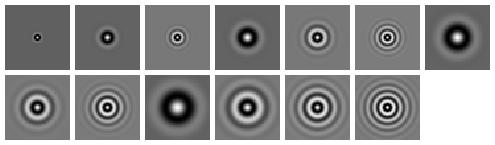
\includegraphics[width=\textwidth,keepaspectratio]{images/vis/vis_02.jpg}
		\subcaption{Schmid-Filterbank}
	\end{subfigure}
	\hfill
	\begin{subfigure}[t]{0.21\textwidth}
		\centering
		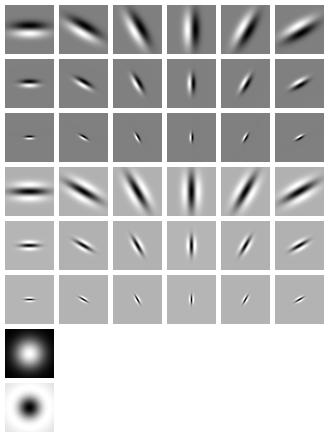
\includegraphics[width=\textwidth,keepaspectratio]{images/vis/vis_03.jpg}
		\subcaption{Maximum Response-Filterbank}
	\end{subfigure}
	\caption{Darstellung dreier Filterbänke, aus \cite{visgeo}}
	\label{fig:filterbank}
\end{figure}

Die Besonderheit der Maximum Response-Filterbank besteht daraus, dass sie zwar 38 Filtern besitzt, nach der Anwendung der Konvolution aber alle bis auf die 6 Filter mit der stärksten Reaktion auf die Eingabe an den k-Means-Algorithmus weitergegeben werden. Zusätzlich werden immer die rotationsinvarianten Filter genutzt.

\iffalse
% TODO Remove?
\section{Kratererkennung}
\label{sec:crater_detection}

In \cite{bandeira_10} und dessen Fortsetzung \cite{bandeira_12} wird ein neuer Ansatz zur Kratererkennung vorgestellt. Zuvor wurden diese meist manuell katalogisiert, dies resultierte darin, dass nur die größten Krater dokumentiert wurden, oder darin, dass nur vergleichsweise kleine Bereiche innerhalb eines akzeptablen Zeitraums verarbeitet werden konnten. Daher legen die Autoren insbesondere Wert auf die korrekte Erkennung von kleineren Kratern.

Die erarbeitete Vorgehensweise beginnt damit, dass über einen möglichst effizienten Algorithmus (hier der Algorithmus von Urbach \etal \cite{urbach_stepinski_2009}) eine Vorsortierung von Krater-Kandidaten berechnet wird. Als Alternative zu diesem Algorithmus werden \cite{bandeira_07} und \cite{salamuniccar_10} genannt.

Der genutzte Algorithmus ist zwar relativ effizient, da er parallel alle Merkmale eliminiert, die nicht auf Krater hindeuten. Frühere Algorithmen hingegen griffen meist auf eine Brute-Force-Methode zurück. Zur Erkennung von Krater (\bzw Krater-Kandidaten) wird hier die Tatsache genutzt, dass diese auf Abbildungen meisten aus nebeneinander liegenden, starken Schatten- und Spitzlicht-Regionen bestehen.

Nach dieser Vorsortierung und Pre-Processing Schritten (in Form von Histogramm-Optimierung) werden in \cite{bandeira_10, bandeira_12} neun Bitmasken (siehe \figurename~\ref{fig:BDS12_01}) in verschiedenen Positionen, Größen und Ausrichtungen über die Kandidaten gelegt. Die Wahrscheinlichkeit, dass der Kandidat ein Krater ist, berechnet sich aus der Übereinstimmung zwischen den Bitmasken und dem eigentlichen Kandidatenbild. Abschließend werden die Ergebnisse mithilfe eines angepassten AdaBoost Algorithmus optimiert. Das Post-Processing besteht aus der Eliminierung von ungewöhnlich geformten Kratern.

\begin{figure}[h!]
	\centering
	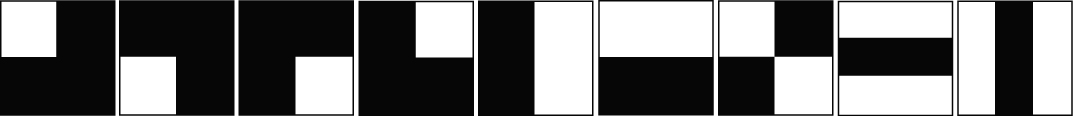
\includegraphics[width=.8\textwidth,keepaspectratio]{images/BDS12/BDS12_01.png}
	\caption{Die neun, zur Merkmalsextrahierung genutzen Bitmasken, aus \cite{bandeira_12}}
	\label{fig:BDS12_01}
\end{figure}

In \figurename~\ref{fig:BDS12_02} sind die von AdaBoost ausgewählten, am stärksten gewichteten Bitmasken-Überlagerungen dargestellt. Es ist zu beachten, dass der Krater im Hintergrund nur ein Beispiel ist, und nicht alle Krater, die von den jeweiligen Bitmasken überlagert werden, darstellt.

\begin{figure}[h!]
	\centering
	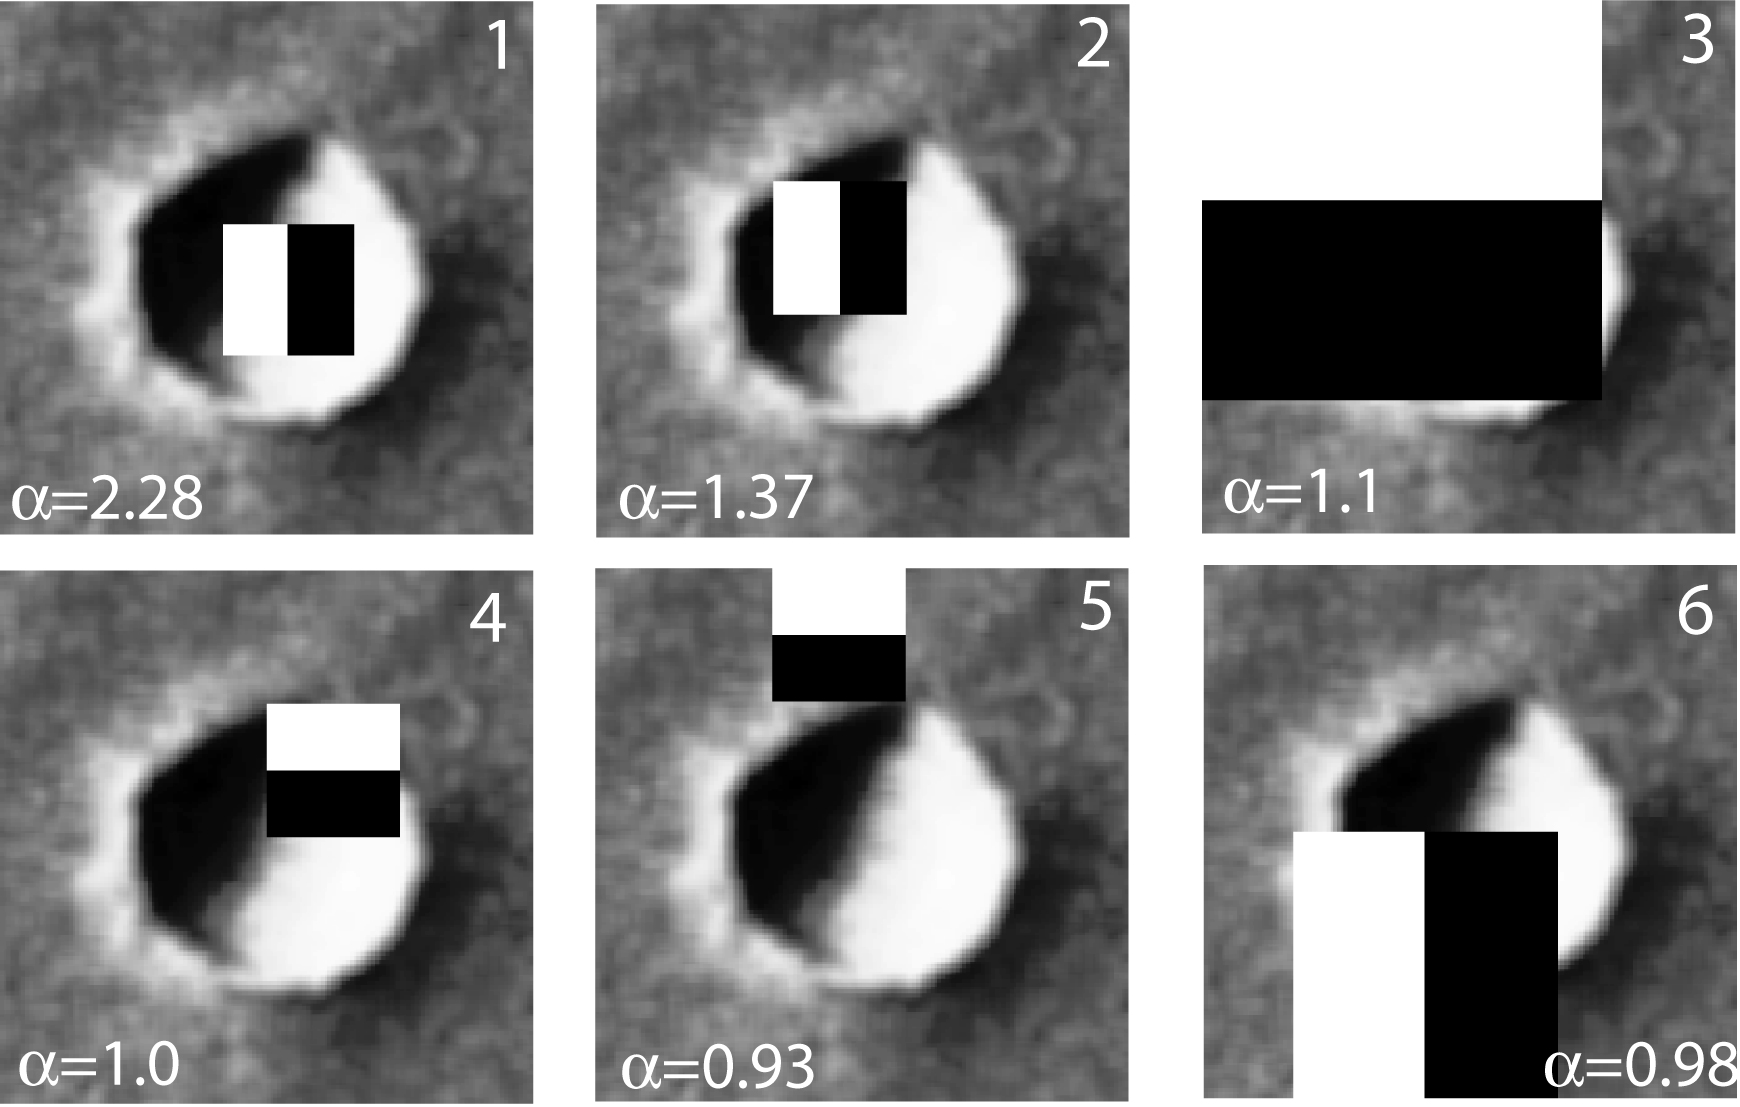
\includegraphics[width=.5\textwidth,keepaspectratio]{images/BDS12/BDS12_02.png}
	\caption{Die sechs am stärksten gewichteten Bitmasken, aus \cite{bandeira_12}}
	\label{fig:BDS12_02}
\end{figure}

\subsection{Kratererkennung über Neuronale Netze}
\label{ssec:crater_detection_nn}
Auf der Basis des erwähnten, automatisch generierten Marskrater-Datensatz, wird in \cite{cohen_16} ein neuronales Netzwerk daraufhin trainiert, selbst unterscheiden zu können, ob ein Kraterkandidat auch wirklich ein Krater ist. Die Architektur des Netzwerkes ist in \figurename~\ref{fig:CLLD16_01} zu sehen. Zur Evaluierung der Ergebnisse wird hier das 10-fache Kreuzvalidierungsverfahren genutzt. Dies bedeutet, dass der Eingabedatensatz zehn-geteilt wird, und jeweils neun Teile zum trainieren und ein Teil zum Evaluieren genutzt wird. Das Ergebnis ist der Durchschnitt der jeweiligen F1-Scores.

\begin{figure}[H]
	\centering
	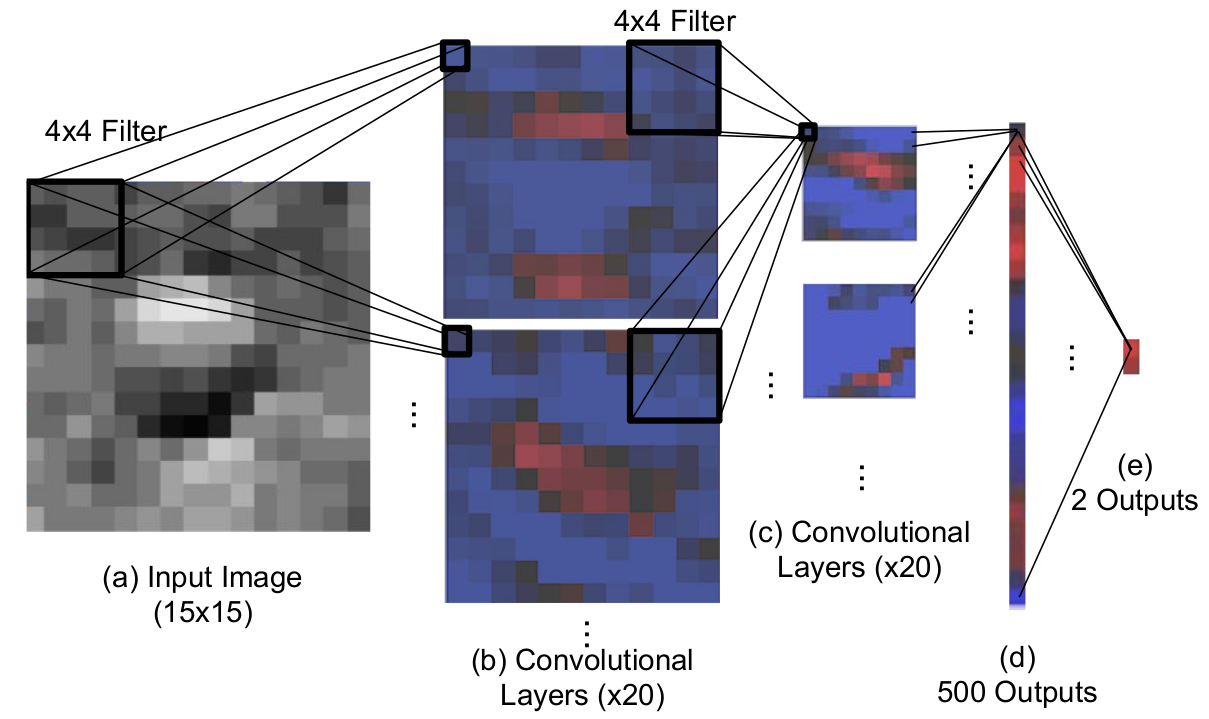
\includegraphics[width=.5\textwidth,keepaspectratio]{images/CLLD16/CLLD16_01.png}
	\caption{Die Architektur des Netzwerkes, aus \cite{cohen_16}}
	\label{fig:CLLD16_01}
\end{figure}

Der Unterschied zwischen dieser Methode und dem hier vorgestellten Ansatz besteht darin, dass in dieser Methode nur bewertet wird, ob Kraterkandidaten wirkliche Krater sind oder nicht, während hier ein Ansatz entwickelt wird, der aus einer kompletten Aufnahme der Marsoberfläche einzelne Krater(kandidaten) erkennt.

%\iffalse
\subsection{Vergleich der Methoden}
\label{ssec:crater_detection_comparision}

Die drei genannten Algorithmen (Urbach '09 \cite{urbach_stepinski_2009}, Bandeira '10 \cite{bandeira_10} und Cohen '16 \cite{cohen_16}) wurden alle auf der selben Aufnahme der HRSC angewandt. Eine genauere Beschreibung und der Vergleich anhand dieser Aufnahme findet sich in Abschnitt~\ref{sec:comparision}.
\fi
